\documentclass[oneside,openright,a4paper,12pt]{abntex2}

\usepackage[english,brazilian]{babel}
\usepackage[utf8]{inputenc}
\usepackage{indentfirst}
\usepackage[T1]{fontenc}
\usepackage{microtype} 
\usepackage{lmodern}
\usepackage[top=20mm, bottom=20mm, left=20mm, right=20mm]{geometry}
\usepackage{framed}
\usepackage{booktabs}	   		% Pacote para deixar tabelas mais bonitas.
\usepackage{color}				% Pacote de Cores
\usepackage{hyperref}			% Pacotes para Hiperlinks
\usepackage{graphicx}			% Pacote de imagens
\definecolor{shadecolor}{rgb}{0.8,0.8,0.8}

\definecolor{blue}{RGB}{41,5,195}



% --- 
% Espaçamentos entre linhas e parágrafos 
% --- 

% O tamanho do parágrafo é dado por:
\setlength{\parindent}{1.3cm}

% Controle do espaçamento entre um parágrafo e outro:
\setlength{\parskip}{0.2cm}  % tente também \onelineskip



% ----
% Início do documento
% ----
\begin{document}

	
	% Retira espaço extra obsoleto entre as frases.
	\frenchspacing 
	
	% ----------------------------------------------------------
	% ELEMENTOS TEXTUAIS
	% ----------------------------------------------------------
	\imprimircapa


	\chapter{Memorial}
Saudações,

Venho por meio deste relatar minhas motivações pessoais para ingresso à Residência Pedagógica. 



Atenciosamente,

xxxx  xxxx
	\begin{anexosenv}
	\partanexos
	\begin{figure}
		
\includegraphics[width=\linewidth]{anexos/rg_frente.jpg}
		\caption[rg frente]{Frente do RG.}
		\label{fig:mv1}
	\end{figure}
	
	\begin{figure}
		
\includegraphics[width=\linewidth]{anexos/rg_verso.jpg}
		\caption[rg verso]{Verso do RG com CPF.}
		\label{fig:mv2}
	\end{figure}
	
	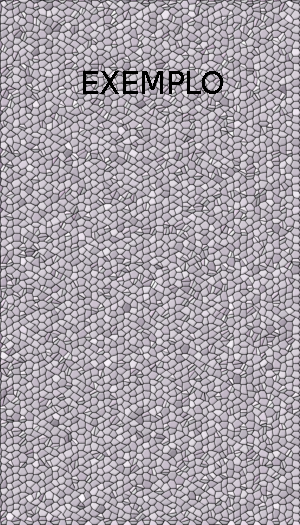
\includepdf[pages=-]{anexos/pdf_exemplo.pdf}
	
	
\end{anexosenv}
	\cleardoublepage
	
	
	
\end{document}